\everymath{\displaystyle}
\documentclass{beamer}
% \documentclass[handout]{beamer}

%\usepackage[pdftex]{color,graphicx}
\usepackage{amsmath,amssymb,amsfonts}

\mode<presentation>
{
  % \usetheme{Darmstadt}
  % \usetheme[hideothersubsections]{Hannover}
  % \usetheme[hideothersubsections]{Goettingen}
  \usetheme[hideothersubsections, right]{Berkeley}

  \usecolortheme{seahorse}
  % \usecolortheme{dolphin}
  \usecolortheme{rose}
  % \usecolortheme{orchid}

  \useinnertheme[shadow]{rounded}

  \setbeamercovered{transparent}
  % or whatever (possibly just delete it)
}

\mode<handout>{
  \setbeamercolor{background canvas}{bg=black!5}
  \usepackage{pgfpages}
  \pgfpagesuselayout{4 on 1}[a4paper,border shrink=5mm, landscape]
}

\usepackage[brazilian]{babel}
% or whatever

% \usepackage[latin1]{inputenc}
\usepackage[utf8]{inputenc}
% or whatever

\usepackage{times}
%\usepackage[T1]{fontenc}
% Or whatever. Note that the encoding and the font should match. If T1
% does not look nice, try deleting the line with the fontenc.


\title%[] % (optional, use only with long paper titles)
{Problema, Hipóteses e Variáveis}

\subtitle
{} % (optional)

\author%[] % (optional, use only with lots of authors)
{Felipe Figueiredo}% \and S.~Another\inst{2}}
% - Use the \inst{?} command only if the authors have different
%   affiliation.

\institute[INTO] % (optional, but mostly needed)
{Instituto Nacional de Traumatologia e Ortopedia
}
  % \inst{1}%
  % Department of Computer Science\\
  % University of Somewhere
  % \and
  % \inst{2}%
  % Department of Theoretical Philosophy\\
  % University of Elsewhere}
% - Use the \inst command only if there are several affiliations.
% - Keep it simple, no one is interested in your street address.

\date%[] % (optional)
{}

% \subject{Talks}
% This is only inserted into the PDF information catalog. Can be left
% out. 



% If you have a file called "university-logo-filename.xxx", where xxx
% is a graphic format that can be processed by latex or pdflatex,
% resp., then you can add a logo as follows:

\pgfdeclareimage[height=1.6cm]{university-logo}{../logo}
\logo{\pgfuseimage{university-logo}}



% Delete this, if you do not want the table of contents to pop up at
% the beginning of each subsection:
\AtBeginSubsection[]
%\AtBeginSection[]
{
  \begin{frame}<beamer>{Sumário}
    \tableofcontents[currentsection,currentsubsection]
  \end{frame}
}


% If you wish to uncover everything in a step-wise fashion, uncomment
% the following command: 

% \beamerdefaultoverlayspecification{<+->}


\begin{document}

\begin{frame}
  \titlepage
\end{frame}

\begin{frame}{Sumário}
  \tableofcontents
  % You might wish to add the option [pausesections]
\end{frame}


%% Template
% \section{}

% \subsection{}

% \begin{frame}{}
%   \begin{itemize}
%   \item 
%   \end{itemize}
% \end{frame}

% \begin{frame}
%   \begin{columns}
%     \begin{column}{5cm}
%     \end{column}
%     \begin{column}{5cm}
%     \end{column}
%   \end{columns}
% \end{frame}

% \begin{frame}{}
%   \includegraphics[height=0.4\textheight]{file1}
%   \includegraphics[height=0.4\textheight]{file2}
%   \includegraphics[height=0.4\textheight]{file3}
%   \begin{figure}
%     \caption{}
%   \end{figure}
% \end{frame}

% \begin{frame}{}
%   \begin{definition}
%   \end{definition}
%   \begin{example}
%   \end{example}
%   \begin{block}{Exercício}
%   \end{block}
% \end{frame}

\section{Discussão da aula passada}

% \subsection{Discussão da aula passada}

\begin{frame}{Discussão da aula passada}
  \begin{block}{}
    Discussão da leitura obrigatória da aula passada
  \end{block}
\end{frame}

\section{Problema}

\begin{frame}
  \begin{center}
    Tema $\Rightarrow$ Problema $\Rightarrow$ Hipótese $\Rightarrow$ Variável

    \bigskip
    \visible<2->{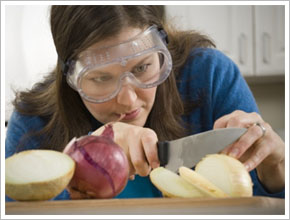
\includegraphics[width=0.8\textwidth]{Hipoteses_variaveis/cebola}}
  \end{center}
\end{frame}

\begin{frame}
  \begin{exampleblock}{Situação clínica 1}
    \footnotesize
    Uma mulher de 19 anos chega em casa do trabalho com sinusite maxilar aguda.

    \bigskip
    Seu médico acabou de ler sobre um tratamento com antibiótico de 3 dias, em contraponto ao tradicional de 10 dias.

    \bigskip
    Ele imagina se deveria prescrever este tratamento para esta paciente.
  \end{exampleblock}

  \vfill
  \scriptsize
  \hfill \href{https://acpjc.acponline.org/Content/123/3/issue/ACPJC-1995-123-3-A12.htm}
      {Richardson et al, 1995}
\end{frame}

\begin{frame}
  \begin{exampleblock}{Situação clínica 2}
    \footnotesize
    Uma mulher de 44 anos com diagnóstico recente de câncer no ovário comparece à emergência com dispnéia e desconforto inspiratório no peito.

    \bigskip
    O exame de ventilação-perfusão retorna ``indeterminado''.

    \bigskip
    O médico da emergência pede sua opinião ``agora que o embolismo foi descartado''.
  \end{exampleblock}

  \vfill
  \scriptsize
  \hfill \href{https://acpjc.acponline.org/Content/123/3/issue/ACPJC-1995-123-3-A12.htm}
      {Richardson et al, 1995}
\end{frame}

\begin{frame}
  \begin{exampleblock}{Situação clínica 3}
    \footnotesize
    Uma professora aposentada de 69 anos vai à consulta de retorno após apresentar insuficiência cardíaca congestiva um mês atrás.

    \bigskip
    Após o médico verificar o progresso, ela pergunta ao médico qual é seu prognóstico.
  \end{exampleblock}

  \vfill
  \scriptsize
  \hfill \href{https://acpjc.acponline.org/Content/123/3/issue/ACPJC-1995-123-3-A12.htm}
      {Richardson et al, 1995}
\end{frame}

\begin{frame}{Problema de pesquisa}
  \begin{itemize}
    \footnotesize
  \item Questão não resolvida, lacuna no conhecimento
    \bigskip
  \item Assunto que se precisa provar ou desenvolver
    \bigskip
  \item Vinculado (e restrito) a um Tema
    \bigskip
  \item Nosso ``ganha-pão''
  \end{itemize}
\end{frame}

\begin{frame}{Exemplo}
  \begin{exampleblock}{Exemplo}
    \begin{center}
      
\includegraphics[width=.95\textwidth]{Metodos/case-series}
    \end{center}
  \end{exampleblock}

  \vfill
  \scriptsize
  \hfill \href{http://dx.doi.org/10.4314/ahs.v12i4.25}{Abu-Zidan, Abbas e Hefny 2012}
\end{frame}

\begin{frame}{Exemplo}
  \begin{exampleblock}{Exemplo}
    \small
    {\bf Tema:} ``O conceito de série de casos na literatura''

    \bigskip

    {\bf Problema:} ``Qual é o número de casos que define um estudo de caso ou uma série de casos?''
  \end{exampleblock}

  \vfill
  \scriptsize
  \hfill \href{http://dx.doi.org/10.4314/ahs.v12i4.25}{Abu-Zidan, Abbas e Hefny 2012}
\end{frame}

\begin{frame}{Exemplo}
  \begin{exampleblock}{Exemplo}
    \small
    {\bf Tema: }``Complicações após transplante de fígado''

    \bigskip

    {\bf Problema:} ``Qual é o regime imunosupressor mais eficaz para previnir a rejeição após um transplante de fígado?''
  \end{exampleblock}

  \vfill
  \scriptsize
  \hfill \href{https://doi.org/10.1002/14651858.cd011639.pub2}{Rodríguez‐Perálvarez et al, 2017}
\end{frame}

\begin{frame}{Exemplo}
  \begin{exampleblock}{Exemplo}
    \small
    {\bf Tema: }``Tratamentos para dor no ombro''

    \bigskip

    {\bf Problema:} ``Acupuntura é um tratamento eficaz e seguro para dor no ombro?''
  \end{exampleblock}

  \vfill
  \scriptsize
  \hfill \href{https://doi.org/10.1002/14651858.CD005319}{Green, Buchbinder e Hetrick, 2005}
\end{frame}

\begin{frame}
  \begin{center}
  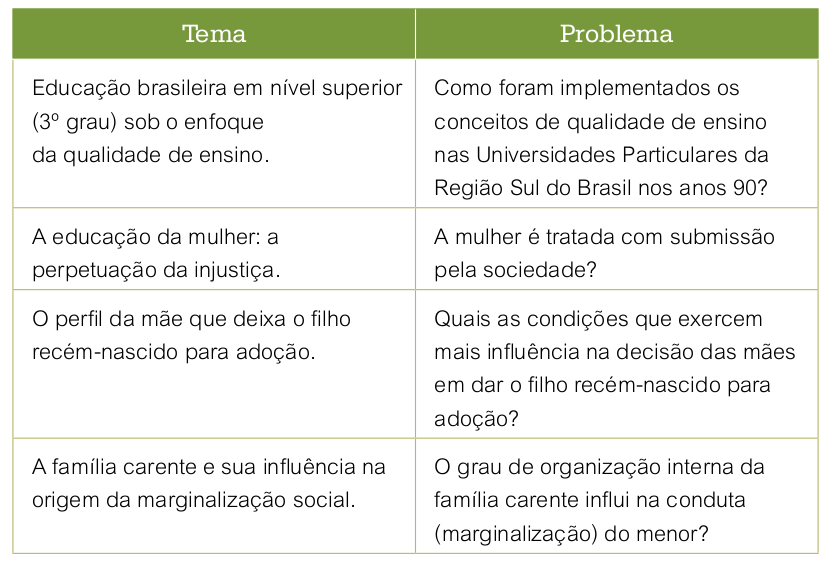
\includegraphics[height=0.8\textheight]{Hipoteses_variaveis/tema_problema}
\end{center}

  \vfill
  \scriptsize
  \hfill Fonte: Prodanov, 2013
\end{frame}

\begin{frame}{Formulação do Problema}
O problema é:
  \begin{itemize}
    \footnotesize
  \item original?
    \bigskip
  \item relevante?
    \bigskip
  \item viável (recursos, tempo, etc)?
  \end{itemize}

  \vfill
  \scriptsize
  \hfill Prodanov, 2013
\end{frame}

\begin{frame}{Fontes de problemas clinicamente relevantes}
  \begin{itemize}
    \footnotesize
  \item Evidência clínica
    \medskip
  \item Diagnóstico
    \medskip
  \item Prognóstico
    \medskip
  \item Terapia
    \medskip
  \item Prevenção
    \medskip
  \item Educação
  \end{itemize}

  \vfill
  \scriptsize
  \hfill \href{https://acpjc.acponline.org/Content/123/3/issue/ACPJC-1995-123-3-A12.htm}
      {Richardson et al, 1995}
\end{frame}

\begin{frame}{Tema x Problema x Hipótese}
  \begin{itemize}
    \footnotesize
  \item Tema: assunto
    \bigskip
  \item Problema: pergunta
    \bigskip
  \item Hipótese: resposta provisória
  \end{itemize}
\end{frame}

\section{Hipóteses}

% \subsection{Hipóteses}

\begin{frame}{Hipóteses}
  \begin{block}{}
    ``(...) um enunciado geral de \alert{relações entre variáveis}
    (fatos, fenômenos).''

    \vfill
    \scriptsize
    \hfill Lakatos, Marconi (2003)
  \end{block}
  % \begin{itemize}
  % \item Solução provisória para o problema
  % \item Caráter explicativo ou preditivo
  % \item Compatível com conhecimento científico (coerência externa)
  % \item Consistência lógica (coerência interna)
  % \item Empiricamente verificável
  % \end{itemize}
  \begin{block}{}
    ``(...) constituem ``respostas'' supostas e provisórias ao
    problema. A principal resposta é denominada hipótese básica,
    podendo ser complementada por outras (...) secundárias.''

    \vfill
    \scriptsize
    \hfill Prodanov, 2013
  \end{block}
\end{frame}

\begin{frame}{Hipóteses}
  \begin{itemize}
    \footnotesize
  \item Declaração que antecipa a relação entre duas ou mais variáveis
    \bigskip
  \item Problema, pesquisa e hipótese estão relacionados
    \bigskip
  \item Deduzida da revisão bibliográfica
    \bigskip
  \item Em estudos quantitativos, pode ser testada (Estatística!)
    \bigskip
  \item {\em ``Aposta''} que o pesquisador faz sobre os possíveis
    resultados
  \end{itemize}

  \vfill
  \scriptsize
  \hfill (Fonte: Prodanov, 2013)
\end{frame}

\begin{frame}{Características das hipóteses}
  \begin{itemize}
    \footnotesize
  \item Consistência lógica
    \medskip
  \item Simplicidade (Navalha de Occam)
    \medskip
  \item Verificabilidade
    \medskip
  \item Embasamento teórico
    \medskip
  \item Especificidade
    \medskip
  \item Plausibilidade
    \medskip
  \item Originalidade
  \end{itemize}

  \vfill
  \scriptsize
  \hfill (Fonte: Prodanov, 2013)
\end{frame}

\begin{frame}{Navalha de Occam}
  \begin{block}{Definição}
    {\em entia non sunt multiplicanda praeter necessitatem}

    \bigskip
    entidades não devem ser multiplicadas sem necessidade
  \end{block}
  \bigskip
  \begin{itemize}
    \footnotesize
  \item William of Ockham (1287 -- 1347)
    \medskip
  \item ``Lei da parcimônia'' ({\em Lex Parsimoniae})
    \medskip
  \item Elegância na simplicidade
  \end{itemize}
\end{frame}

\begin{frame}{Fontes de hipóteses}
  As hipóteses tipicamente surgem de
  \bigskip
  \begin{itemize}
    \footnotesize
  \item Observação
    \medskip
  \item Resultados de outras pesquisas
    \medskip
  \item Teorias
    \medskip
  \item Intuição
  \end{itemize}

  \vfill
  \scriptsize
  \hfill (Fonte: Prodanov, 2013)
\end{frame}

\begin{frame}{Formulação de hipóteses}
  \begin{block}{Atenção}
    Hipóteses não são perguntas, e sim afirmações
  \end{block}

  \begin{exampleblock}{Exemplo}
    \footnotesize
    {\bf Problema:} como o Marketing de patrocínio
    contribui no processo de construção da marca das organizações?

    \begin{itemize}
      \scriptsize
    \item organizações que patrocinam causas éticas, ambientais e
      sociais possuem melhoria de imagem e crescimento de vendas junto
      à comunidade
    \item o marketing de patrocínio fortalece o envolvimento dos
      funcionários com a missão da empresa.
    \end{itemize}

    \vfill
    \scriptsize
    \hfill Prodanov, 2013
\end{exampleblock}
\end{frame}

\section{Variáveis}

\begin{frame}{Variáveis}
  \begin{itemize}
    \footnotesize
  \item Hipóteses também podem ser formuladas como uma conexão causal
    entre duas (ou mais) variáveis
    \bigskip
  \item Se X, então Y
    \bigskip
  \item Variáveis podem
    \begin{itemize}
      \scriptsize
    \item descrever o fenômeno
    \item explicar o fenômeno
    \end{itemize}
  \end{itemize}
\end{frame}

\begin{frame}{Tipos de Variáveis}
  \begin{block}{Definição}
    Variável \alert{dependente} (ou resposta) é a variável a ser
    explicada no estudo.
  \end{block}
  \begin{block}{Definição}
    Variável \alert{independente} (ou explanatória) é a variável que
    serve de suporte na explicação da variabilidade da variável
    resposta.
  \end{block}
\end{frame}

\subsection{Níveis de mensuração}

\begin{frame}{Tipos de Variáveis}
Variáveis podem ser classificadas em duas principais categorias
  \begin{itemize}
  \item Qualitativas (categóricas)
  \item Quantitativas (numéricas)
  \end{itemize}
  \begin{exampleblock}{Exemplo}
    Pressão sistólica (mmHg), altura (cm), sexo (M ou F), grau de
    satisfação com atendimento médico (nota de 1 a 5), perímetro
    abdominal (cm), contagem de leucócitos, número de pessoas na
    família, cor da pele (branco, negro, pardo), etc.
  \end{exampleblock}
\end{frame}

\begin{frame}{Variáveis qualitativas}
Variáveis qualitativas se subdividem em
  \begin{itemize}
  \item<1-2> Nominais
  % \begin{example}
  %   sexo, cor da pele
  % \end{example}

  \item<3-4> Ordinais
  \end{itemize}

  % \begin{example}
  %   satisfação com atendimento médico (nota de 1 a 5)
  % \end{example}

  \begin{exampleblock}{Exemplo}
    Pressão sistólica (mmHg), altura (cm), \only<2>\alert{sexo (M ou
      F)}, \only<4>\alert{grau de satisfação com atendimento médico
      (nota de 1 a 5)}, perímetro abdominal (cm), contagem de
    leucócitos, número de pessoas na família, \only<2>\alert{cor da
      pele (branco, negro, pardo)}, etc.
  \end{exampleblock}
\end{frame}

\begin{frame}{Variáveis quantitativas}
Variáveis quantitativas se subdividem em
  \begin{itemize}
  \item<1-2> Discretas
  \item<3-4> Contínuas
  \end{itemize}
  \begin{exampleblock}{Exemplo}
    \only<4>\alert{Pressão sistólica (mmHg)}, \only<4>\alert{altura
      (cm)}, sexo (M ou F), grau de satisfação com atendimento médico
    (nota de 1 a 5), perímetro abdominal (cm), \only<2>\alert{contagem
      de leucócitos}, \only<2>\alert{número de pessoas na família},
    cor da pele (branco, negro, pardo), etc.
  \end{exampleblock}
\end{frame}

\subsection{VD -- Desfecho}

\subsection{VI -- Exposição ou tratamento}

\begin{frame}{Hipótese x Variáveis}
  \begin{center}
  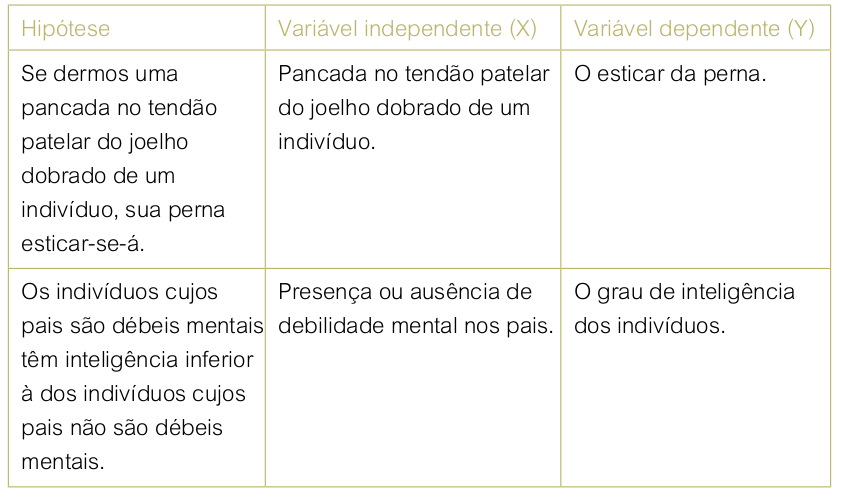
\includegraphics[height=0.8\textheight]{Hipoteses_variaveis/hipotese_variaveis}
\end{center}

  \vfill
  \scriptsize
  \hfill Fonte: Prodanov, 2013
\end{frame}

\section{Formulação sistemática de pergunta -- PICO}

\begin{frame}{PICO}
  \begin{center}
    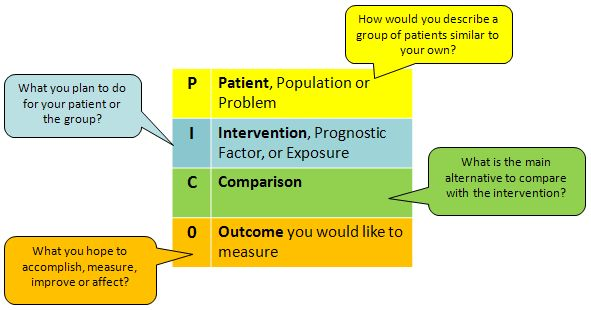
\includegraphics[height=0.8\textheight]{Hipoteses_variaveis/pico}
  \end{center}
\end{frame}

\begin{frame}{Terapia}
  \begin{exampleblock}{Situação clínica 1}
    \scriptsize
    Uma mulher de 19 anos chega em casa do trabalho com sinusite maxilar aguda.
    Seu médico acabou de ler sobre um tratamento com antibiótico de 3 dias, em contraponto ao tradicional de 10 dias.
    Ele imagina se deveria prescrever este tratamento para esta paciente.
  \end{exampleblock}
  \begin{exampleblock}{PICO}
    Em adultos com sinusite maxilar aguda, um tratamento de 3 dias com {\em trimethoprim-sulfamethoxazole} tem a mesma taxa de cura que o tratamento de 10 dias, com menos efeitos adversos e menor custo?
  \end{exampleblock}
  \vfill
  \scriptsize
  \hfill \href{https://acpjc.acponline.org/Content/123/3/issue/ACPJC-1995-123-3-A12.htm}
      {Richardson et al, 1995}
\end{frame}

\begin{frame}{Diagnóstico}
  \begin{exampleblock}{Situação clínica 2}
    \scriptsize
    Uma mulher de 44 anos com diagnóstico recente de câncer no ovário comparece à emergência com dispnéia e desconforto inspiratório no peito.
    O exame de ventilação-perfusão retorna ``indeterminado''.
    O médico da emergência pede sua opinião ``agora que o embolismo foi descartado''.
  \end{exampleblock}
  \begin{exampleblock}{PICO}
    Quando comparada com a angiografia pulmonar, quão bem um resultado indeterminado de ventilação-perfusão descarta o embolismo pulmonar em um paciente com alta probabilidade pré teste?
  \end{exampleblock}
  \vfill
  \scriptsize
  \hfill \href{https://acpjc.acponline.org/Content/123/3/issue/ACPJC-1995-123-3-A12.htm}
  {Richardson et al, 1995}
\end{frame}

\begin{frame}{Prognóstico}
  \begin{exampleblock}{Situação clínica 3}
    \scriptsize
    Uma professora aposentada de 69 anos vai à consulta de retorno após apresentar insuficiência cardíaca congestiva um mês atrás.
    Após o médico verificar o progresso, ela pergunta ao médico qual é seu prognóstico.
  \end{exampleblock}
  \begin{exampleblock}{PICO}
    Qual é a sobrevida média de pacientes com insuficiência cardíaca congestiva, e que características clínicas identificam pacientes com sobrevidas maiores ou menores que a média?
  \end{exampleblock}
  \vfill
  \scriptsize
  \hfill \href{https://acpjc.acponline.org/Content/123/3/issue/ACPJC-1995-123-3-A12.htm}
  {Richardson et al, 1995}
\end{frame}

\section{Aprofundamento}

\subsection{Aprofundamento}

\begin{frame}{Aprofundamento}
  \begin{block}{Leitura obrigatória}
    \begin{itemize}
      \scriptsize
    \item \href{https://doi.org/10.1111/j.1741-6787.2005.00032.x}
      {FINEOUT‐OVERHOLT, Ellen; JOHNSTON, Linda. Teaching EBP: Asking
        searchable, answerable clinical questions. {\bf Worldviews on
          Evidence‐Based Nursing}, v. 2, n. 3, p. 157-160, 2005.}
    \end{itemize}
  \end{block}
  \begin{block}{Leitura recomendada}
    \begin{itemize}
      \tiny
    \item \href{https://doi.org/10.1007/s12630-008-9007-4}
      {THABANE, Lehana et al. Posing the research question: not so
        simple. {\bf Canadian Journal of Anesthesia/Journal canadien
          d'anesthésie}, v. 56, n. 1, p. 71, 2009.}
    \item \href{https://doi.org/10.1542/gr.19-1-2}
      {MOYER, Virginia. Weighing the evidence: PICO questions: What
        are they, and why bother?. {\bf AAP Grand Rounds}, v. 19,
        n. 1, p. 2-2, 2008.}
    \item
      \href{https://acpjc.acponline.org/Content/123/3/issue/ACPJC-1995-123-3-A12.htm}
      {RICHARDSON, W. Scott et al. The well-built clinical question: a
        key to evidence-based decisions. {\bf ACP journal club},
        v. 123, n. 3, p. A12-A12, 1995.}
      \scriptsize
    \item Livro texto: seções {\bf 4.1, 4.3, 4.4}
    \end{itemize}
  \end{block}
\end{frame}

\end{document}
